\documentclass[11pt]{article}

\usepackage[a4paper,margin=1in]{geometry}
\usepackage{amsmath,amssymb,amsthm,mathtools}
\usepackage{booktabs,array,tabularx}
\usepackage{graphicx}
\usepackage[numbers,sort&compress]{natbib}
\usepackage[hidelinks]{hyperref}
\usepackage{enumitem}
\usepackage{xcolor}
\setlist{itemsep=2pt,topsep=4pt}

\newtheorem{proposition}{Proposition}
\newtheorem{lemma}[proposition]{Lemma}
\theoremstyle{definition}
\newtheorem{definition}{Definition}
\theoremstyle{remark}
\newtheorem{remark}{Remark}

\newcommand{\artanh}{\operatorname{artanh}}
\newcommand{\gd}{\operatorname{gd}}
\newcommand{\sech}{\operatorname{sech}}
\newcommand{\Erad}{E_{\mathrm{rad}}}

\newenvironment{boxed-note}{\par\medskip\noindent\begin{tabular}{|p{0.95\textwidth}|}\hline\vspace{-2pt}}{\\\hline\end{tabular}\par\medskip}

\title{The Two-Face Problem:\\[2pt]
\large A Practical Guide to Translating Binary-Partition Formulas Across Disciplines}
\author{Elias De Jes\'us\\
\small Independent Researcher\\
\small ORCID: 0009-0007-0190-9143 \quad \texttt{dejesuselias10@gmail.com}}
\date{Revision 3, October 2026\\ \small (Revision 2: April 2026)}

\begin{document}
\maketitle

\begin{abstract}
Many disciplines use formulas that look structurally related but behave differently,
because they are written in different variables, on different domains, or under different
boundary conditions. This guide gives a practical way to diagnose such cases when the
quantities involved form a two-channel budget $a+b=1$. Every such budget lies on the same
semicircle (the Thales arc), $(a-b)^2+4ab=(a+b)^2$, and the guide supplies an exact
dictionary between the coordinates commonly used on it: the bounded asymmetry and Fisher
angle, the unbounded rapidity (half the log-odds), and the radial response coordinate;
the bounded angle and the rapidity are linked by the Gudermannian.

Revision 3 reorganizes the guide around one principle: \emph{the arc is universal, but how
it is read is supplied by the mechanism.} An \emph{instantiation} fixes, from the domain and
before any comparison, what $a$ and $b$ are; whether the budget is actually closed or leaks;
whether the coupling $\sqrt{ab}$ is realized or only potential; which coordinate is native,
judged by the domain's own composition law; and whether orientation matters. Translations
between coordinates are exact but, applied to a known formula, they are normal forms rather
than discoveries; a reading earns empirical content only by passing an over-determination
test (a family fit, an independently determined law, cross-domain recurrence under a fixed
normalization, or compression). A worked analysis of the SXS binary-black-hole catalog
shows the procedure at work: the coordinate chosen from the physics (the symmetric mass
ratio $\eta=h^2$) gives the most compact description of radiated energy and final spin out of
sample; the radiated-energy leakage is consistent with, though not a sharp test of, the
test-particle limit (ISCO binding energy times the coupling); and the recoil is compactly
written as coupling times asymmetry, reproducing the known maximum near 175~km/s.

The empirical ``equipartition differential'' reported in Revision 2 is withdrawn: a null
simulation reproduces it from unequal bin widths alone, and it does not replicate on the
current SXS catalog. The heuristic sections on a ``dimensional selection'' from a powered
metric family and on ``Pythagorean power distributions'' are removed. An error in one
worked translation (the generating function $G(t)$) is corrected.
\end{abstract}

\noindent\textbf{Keywords:} binary partition; Thales arc; Gudermannian; Fisher metric;
rapidity; exponential family; leakage; instantiation; normal form; falsifiability;
SXS catalog.

\tableofcontents

% =====================================================================
\section{The problem, and what this revision changes}\label{sec:intro}

Across the sciences one meets formulas that look related but behave differently. A
normalized occupation is bounded, a Boltzmann factor is not; a Lorentz factor is hyperbolic,
an inverse-square law is radial. This guide addresses a limited version of that observation.
When the quantities form a conserved two-channel budget $a+b=1$, the budget leaves one
degree of freedom, and several familiar formulas turn out to be the same state written in
different coordinates. Translating between those coordinates can show that an apparent
mismatch is only a change of variables, or that it is a real difference that survives
translation. Both outcomes are useful.

\paragraph{What Revision 3 changes.} Revision 2 presented three fixed ``descriptions'' of the
partition state (Fisher, Poincar\'e, Compound) and chose among them by which one made a
formula look simplest. That criterion is subjective, and it cannot distinguish a coordinate
that is merely available from one the domain actually uses. Revision 3 replaces it with
three ideas developed since:
\begin{enumerate}\sloppy
\item \emph{Instantiation} (Section~\ref{sec:instantiation}): the arc is a universal
constraint locus, and the domain supplies how it is read --- embedding, closure, coupling
type, native coordinate, orientation, dynamics --- fixed before comparison.
\item \emph{Normal forms versus tests} (Section~\ref{sec:tests}): an exact translation of a
known formula is a normal form; a claim acquires content only by passing an
over-determination test~\cite{DeJesus2026EP}.
\item \emph{Leakage} (Section~\ref{sec:leakage}): when the budget is not closed, the state
lives in a half-disk rather than on the arc~\cite{DeJesus2026Fiber,DeJesus2026HL}.
\end{enumerate}
The changes in the empirical and heuristic material are listed in
Section~\ref{sec:withdrawn}.

\paragraph{Epistemic tiers.} \textbf{Tier 1}: exact identities and translations.
\textbf{Tier 2}: readings that have passed an over-determination test in a stated setting,
or empirical results in a stated dataset. \textbf{Tier 3}: interpretive or speculative
claims. Following~\cite{DeJesus2026CG}, a Tier-1 translation is never by itself evidence
for shared physics.

\begin{center}
\fbox{\begin{minipage}{0.92\textwidth}
\textbf{Quick start.}
(1) Identify the two channels and check whether their total is conserved.
(2) Instantiate the arc from the mechanism (Section~\ref{sec:instantiation}) \emph{before}
looking at data.
(3) Translate with the dictionary (Section~\ref{sec:dictionary}).
(4) Classify the result: exact translation, partial correspondence, mixed object, or
mismatch (Section~\ref{sec:pairs}).
(5) If you want more than a re-expression, run an over-determination test
(Section~\ref{sec:tests}) and report it, including failures.
\end{minipage}}
\end{center}

% =====================================================================
\section{The arc}\label{sec:arc}

\subsection{The binary partition and its coordinates}
A two-channel budget with shares
\begin{equation}\label{eq:partition}
a+b=1,\qquad a,b\in(0,1)
\end{equation}
leaves one degree of freedom. We use the \emph{signed} asymmetry
\begin{equation}\label{eq:chi}
\chi=a-b\in(-1,1),\qquad a=\tfrac{1+\chi}{2},\quad b=\tfrac{1-\chi}{2}.
\end{equation}
Revision 2 used $|2a-1|$. The signed form is preferred because many mechanisms distinguish
the two channels (Section~\ref{sec:instantiation}); symmetric quantities below are even in
$\chi$ and cannot do so. Define
\begin{equation}\label{eq:thales}
h=\sqrt{ab},\qquad L=\frac{a-b}{2},\qquad R=\frac{1}{1-\chi^2}=\frac{1}{4h^2},
\qquad \xi=\artanh\chi,\qquad \theta=\arcsin\chi,
\end{equation}
the altitude (geometric mean), half-asymmetry, response, rapidity and Fisher angle.

\begin{proposition}[The Thales arc; Tier 1]\label{prop:arc}
For any nonnegative $a,b$,
\begin{equation}\label{eq:circle}
(a-b)^2+4ab=(a+b)^2 .
\end{equation}
Hence on a closed budget $L^2+h^2=\tfrac14$ and $\chi^2+(2h)^2=1$: every binary partition lies
on the same semicircle of diameter $a+b$.
\end{proposition}

The proof is one line of algebra. The consequence matters for interpretation: lying on the
arc is automatic, so it is never evidence that two domains share structure. The name refers
to Thales' theorem: $h$ is the altitude of the right triangle inscribed in the semicircle of
diameter $a+b$.

\subsection{The mean hierarchy}
The arithmetic, geometric and harmonic means of the shares are $\tfrac12$, $h$ and $2h^2$.

\begin{proposition}[Adjacent-gap ratio; Tier 1]\label{prop:means}
\[
\frac{\mathrm{AM}-\mathrm{GM}}{\mathrm{GM}-\mathrm{HM}}=\frac{1/2-h}{h-2h^2}
=\frac{1}{2h}=\frac{1}{\sqrt{1-\chi^2}} .
\]
\end{proposition}

\subsection{Two dual coordinates: shares and forces}
For a binary random variable with success probability $a$, the share $a$ (equivalently
$\chi$) is the \emph{mean} parameter of the Bernoulli family, and the log-odds
$\log(a/b)=2\xi$ is its \emph{natural} parameter. The two are related by
\begin{equation}\label{eq:legendre}
\chi=\tanh\xi,\qquad \frac{d\xi}{d\chi}=\frac{1}{1-\chi^2}=R,
\end{equation}
the Legendre correspondence of the exponential family~\cite{AmariNagaoka2000}. This is the
standard reason a bounded coordinate and an unbounded one appear together. The bounded face
records \emph{how much} of the budget each channel holds. The unbounded face records the
conjugate \emph{force}: a chemical-potential difference, a log-likelihood ratio, an
impedance ratio, or a rapidity. The response $R$ is the exchange rate between them: the
force needed per unit change of share. It grows without bound near the boundary, which is
the precise sense in which pushing an already lopsided split further is costly.

% =====================================================================
\section{Metrics and the translation dictionary}\label{sec:dictionary}

\subsection{Three metrics on one line}
Three metrics on $\chi\in(-1,1)$ recur in applications. Each has a flat (arc-length)
coordinate:
\begin{align}
ds_F^2&=\frac{da^2}{a}+\frac{db^2}{b}=\frac{d\chi^2}{1-\chi^2}=d\theta^2,
&&\theta=\arcsin\chi\in(-\tfrac\pi2,\tfrac\pi2),\label{eq:fisher}\\
ds_P^2&=\frac{d\chi^2}{(1-\chi^2)^2}=d\xi^2,&&\xi=\artanh\chi\in\mathbb R,\label{eq:rapid}\\
ds_C^2&=\frac{\chi^2\,d\chi^2}{(1-\chi^2)^4}=dy^2,&&y=\tfrac R2\in[\tfrac12,\infty).\label{eq:radial}
\end{align}
The first is the Fisher metric of the Bernoulli family~\cite{Fisher1925,Rao1945}. The second
is the one-dimensional hyperbolic (rapidity) metric. The third is the radial metric of
Revision 2; it is degenerate at $\chi=0$, so $y$ is a chart on each half $\chi>0$ and
$\chi<0$ separately. They are related exactly by
\begin{equation}\label{eq:inversion}
ds_C^2=J^2\gamma^2\,ds_P^2,\qquad J=\sinh\xi,\quad\gamma=\cosh\xi .
\end{equation}

\begin{remark}[What distinguishes them; Tier 1]\label{rem:flat}
Every one-dimensional metric is flat, so the three differ not in curvature but in two
things: whether the boundary $|\chi|\to1$ lies at finite distance (Fisher) or infinite
distance (rapidity, radial), and which coordinate is affine. Which metric is physically
relevant is supplied by the domain (Section~\ref{sec:instantiation}). A kinetic term written
with the Fisher denominator and expressed in $\xi$ carries a residual $\sech^2\xi$ weight;
that weight reflects the metric--coordinate pairing, not domain physics~\cite{DeJesus2026EP}.
\end{remark}

\subsection{The Gudermannian bridge and the dictionary}
The bounded angle and the rapidity are linked by the Gudermannian:
\begin{equation}\label{eq:gd}
\begin{gathered}
\theta=\gd\xi=\arctan(\sinh\xi),\\
\sin\theta=\tanh\xi=\chi,\quad \cos\theta=\sech\xi=2h,\quad \tan\theta=\sinh\xi,\quad\sec\theta=\cosh\xi .
\end{gathered}
\end{equation}

\begin{table}[ht]
\centering\small
\caption{The translation dictionary on a closed budget ($\chi\ge0$ branch shown for the
radial column; for $\chi<0$ odd quantities change sign). All entries are exact (Tier 1) and
are verified in \texttt{verify\_rev3.py}.}
\label{tab:dictionary}
\begin{tabular}{@{}lccc@{}}
\toprule
Quantity & Fisher angle $\theta$ & Rapidity $\xi$ & Radial $y=R/2$\\
\midrule
Asymmetry $\chi$ & $\sin\theta$ & $\tanh\xi$ & $\sqrt{1-1/(2y)}$\\
Altitude $h$ & $\tfrac12\cos\theta$ & $\tfrac12\sech\xi$ & $1/\sqrt{8y}$\\
$J=\chi/\sqrt{1-\chi^2}$ & $\tan\theta$ & $\sinh\xi$ & $\sqrt{2y-1}$\\
$\gamma=1/(2h)$ & $\sec\theta$ & $\cosh\xi$ & $\sqrt{2y}$\\
Response $R$ & $\sec^2\theta$ & $\cosh^2\xi$ & $2y$\\
Log-odds $\log(a/b)$ & $2\artanh(\sin\theta)$ & $2\xi$ & $2\,\mathrm{arccosh}\sqrt{2y}$\\
\bottomrule
\end{tabular}
\end{table}

A useful companion is the square-root (Bhattacharyya) angle $\varphi=\arcsin\sqrt a$, which
embeds the partition on a circle as $(\sqrt a,\sqrt b)=(\sin\varphi,\cos\varphi)$. It
satisfies $\theta=2\varphi-\pi/2$, and the Fisher distance between two partitions is twice
the difference of their $\varphi$ values.

% =====================================================================
\section{Instantiating the arc}\label{sec:instantiation}

The arc is the same for every two-channel budget. What changes from one domain to another is
everything that gives the arc meaning, and none of it comes from the geometry. We call a
specification of those components an \emph{instantiation}.

\begin{definition}[Instantiation]\label{def:inst}
An instantiation of the arc for a mechanism $M$ fixes, from $M$ alone:
\begin{enumerate}[label=(\roman*)]
\item \textbf{Embedding}: what the channels $a$ and $b$ are physically;
\item \textbf{Closure}: whether $a+b$ is conserved, or whether a third channel takes part of
the total (Section~\ref{sec:leakage});
\item \textbf{Coupling type}: whether $2h=2\sqrt{ab}$ is the realized coupling between the
channels, or only the maximum possible coupling (Section~\ref{sec:leakage});
\item \textbf{Native coordinate}: the coordinate in which the domain's own composition law
is additive, or in which its dynamics close;
\item \textbf{Orientation}: whether $M$ distinguishes $a$ from $b$, in which case the signed
$\chi$ (or $\xi$) is required and the symmetric quantities $h$, $R$, $y$ are insufficient;
\item \textbf{Dynamics and landmarks}: what moves the state, and which points $M$ itself
singles out.
\end{enumerate}
\end{definition}

\paragraph{The pre-commitment rule.} An instantiation must be fixed by the mechanism
\emph{before} anything is compared with data or with a target value. Chosen afterwards, the
components carry enough freedom to fit almost anything; this is the threshold-manufacturing
risk of~\cite{DeJesus2026CG}. With the rule in place, every claim has the form ``under the
instantiation supplied by $M$, we expect $X$.'' If $X$ fails, that instantiation is rejected
and the arc is untouched.

\subsection{The native coordinate is decided by composition}
Revision 2 chose a ``native description'' by simplicity of form. Revision 3 uses an
operational criterion: \emph{a coordinate is native to a domain when the domain's own way of
combining two states becomes addition in that coordinate.} Examples:
\begin{itemize}
\item \textbf{Collinear Lorentz boosts.} Einstein addition
$\beta_1\oplus\beta_2=(\beta_1+\beta_2)/(1+\beta_1\beta_2)$ is addition of rapidities and
multiplication of the odds $(1+\beta)/(1-\beta)$, which are the squared Bondi
$k$-factors~\cite{Bondi1964,Varicak1910,DeJesus2026SR}. Rapidity is native.
\item \textbf{Bayesian updating of a binary hypothesis.} Independent evidence multiplies
likelihood ratios, so log-odds $=2\xi$ add. Rapidity is native.
\item \textbf{Resistive impedance mismatch.} For a real load $Z$ on a line of impedance
$Z_0$, the reflection coefficient is $\Gamma=(Z-Z_0)/(Z+Z_0)=\tanh\!\big(\tfrac12\ln(Z/Z_0)\big)$.
Changing reference impedance multiplies impedance ratios, so $\xi=\tfrac12\ln(Z/Z_0)$ adds.
Rapidity is native, and the standing-wave ratio is $e^{2|\xi|}$.
\item \textbf{Cosmic expansion.} Scale factors multiply, so e-folds $N=\ln a$ add. In the
flat matter--$\Lambda$ partition with $a=\Omega_\Lambda$, the rapidity flows at the
constant rate $d\xi/dN=+\tfrac32$ (Section~\ref{sec:examples}).
\item \textbf{Estimation of a proportion.} Here there is no composition of states, and the
native coordinate is fixed instead by the statistics: the Fisher (or Bhattacharyya) angle,
in which the estimation noise is uniform. The estimator $\arcsin\sqrt{\hat p}$ has variance
close to $1/(4n)$ whatever $p$ is (variance stabilization). The Fisher information $8y$ per
trial is the metric weight in the share coordinate, not a composition law.
\end{itemize}
Where no composition law is available, the domain's dynamics or its standard expansions
decide. The SXS analysis of Section~\ref{sec:sxs} is an example: there the native coordinate
is the coupling $h^2=\eta$, the expansion variable of post-Newtonian theory.

\subsection{Constraint types}
The kind of constraint a mechanism imposes tells you which coordinate to expect:

\begin{table}[ht]
\centering\small
\caption{Constraint types and the coordinates they act on (Tier 3: an organizing heuristic,
to be checked for each mechanism).}
\label{tab:constraints}
\begin{tabular}{@{}p{0.2\textwidth}p{0.27\textwidth}p{0.18\textwidth}p{0.27\textwidth}@{}}
\toprule
Constraint & How it acts & Expected coordinate & Examples\\
\midrule
Scarcity / budget & fixes the total $a+b$ & shares $a,b$ or $\chi$ & probabilities, mass fractions\\
Pressure / force & sets the position on the arc & rapidity $\xi$ & Fermi--Dirac (log-odds of occupation $=-(E-\mu)/kT$), voltages\\
Conservation & total fixed while the split changes & motion along the arc & energy exchange $T\leftrightarrow V$\\
Dissipation / friction & drives the split to a rest point & a flow on the arc & relaxation; near equilibrium, flux $\propto$ force~\cite{Onsager1931}\\
\bottomrule
\end{tabular}
\end{table}

% =====================================================================
\section{Leakage and partial coupling}\label{sec:leakage}

\subsection{Open budgets}
Suppose a third channel $Q\ge0$ takes part of a total $E$: $T+V+Q=E$ for two active channels
$T,V\ge0$, with leakage fraction $\lambda=Q/E$~\cite{DeJesus2026Fiber,DeJesus2026HL}.
(We write $\lambda$ here to avoid a clash with the half-asymmetry $L$ of~\eqref{eq:thales}.)
Write $a=T/E$, $b=V/E$, so $a+b=1-\lambda$.

\begin{proposition}[Angle and radius; Tier 1]\label{prop:leak}
With conditional shares $A=a/(1-\lambda)$, $B=b/(1-\lambda)$,
\[
(A-B)^2+4AB=1,\qquad (a-b)^2+4ab=(1-\lambda)^2,\qquad
R_{\rm act}=\frac{1}{4ab}=\frac{R_{\rm cond}}{(1-\lambda)^2}.
\]
\end{proposition}

So the state is a point in a half-disk. The \emph{angle} records the internal exchange
between the two active channels. The \emph{radius} $1-\lambda$ records how much of the
total remains active. Leakage that draws on both channels in proportion moves the point
inward without changing its direction; leakage from one channel also changes the angle.

Two practical consequences follow. First, the closure question (ii) of
Definition~\ref{def:inst} must be asked of every application: if the budget is not closed,
normalizing to $a+b=1$ hides a second variable. Second, the global response $R_{\rm act}$
grows as the active fraction shrinks even when nothing changes internally, so a large
observed response can be produced by leakage alone.

\paragraph{A familiar geometry.} With amplitudes $x=\sqrt a$, $y=\sqrt b$ one has
$(a-b,\,2\sqrt{ab})=(x^2-y^2,\,2xy)$ and $a+b=x^2+y^2$: the arc is the image of a
quarter-circle of amplitudes under squaring. This is the geometry of the Stokes parameters
of two field components~\cite{Stokes1852} and of the Bloch vector of a two-level
system~\cite{Bloch1946}. The leakage picture is the same bookkeeping used for population
leaking out of the computational subspace of a qubit~\cite{WoodGambetta2018}.

\subsection{Realized versus potential coupling}
In optics and two-level systems the vector can also move inward \emph{without} leakage, when
the two channels lose phase coherence while their populations stay fixed. The realized
coupling is then smaller than $\sqrt{ab}$. Because $h$ is defined as $\sqrt{ab}$, it is the
\emph{maximum} coupling the shares allow, and it cannot detect such dephasing. This is
question (iii) of Definition~\ref{def:inst}: whether $2h$ describes an actual interaction or
only an upper bound depends on the mechanism.

\subsection{Scale as a hidden coordinate}
When a family test fails because the extracted dynamics depend on the total $S=a+b$, the
correct conclusion is that the state is two-dimensional (share and scale). The worked
example is one-loop gauge-coupling running: the extracted potential scales as $S^2$, so no
autonomous one-dimensional partition potential exists~\cite{DeJesus2026EP}. Leakage and
gauge running are therefore two instances of the same closure question.

% =====================================================================
\section{Normal forms and over-determination tests}\label{sec:tests}

\begin{remark}[Why translation alone cannot fail]\label{rem:tautology}
Translating a known formula into another coordinate is exact and always succeeds. In the
same way, extracting an effective potential from one known trajectory reconstructs that
trajectory exactly, because the free function absorbs the input~\cite{DeJesus2026EP}. Such
results are \emph{normal forms}: useful for classification, but not evidence of a mechanism.
\end{remark}

A reading of the arc acquires empirical content only when it is asked to do something it was
not built to do. Four routes, from~\cite{DeJesus2026EP}:
\begin{enumerate}\sloppy
\item \textbf{Family or held-out test}: one law must fit a whole family of cases, including
cases not used to fix it, with the residual reported.
\item \textbf{Independent determination}: a principle from the domain (an action, a free
energy, a conservation law, a limiting case) fixes the law, which then predicts the data.
\item \textbf{Cross-domain recurrence under a fixed normalization}, declared before the
comparison.
\item \textbf{Compression}: a law with few parameters replaces a long description.
\end{enumerate}
Each route can fail, and a failure is informative: it classifies the domain (for example,
as not governed by an autonomous one-dimensional law) rather than refuting the arc.

% =====================================================================
\section{Worked translations}\label{sec:pairs}

The pairs below are exact translations (Tier 1). Each is a normal form in the sense of
Remark~\ref{rem:tautology}. The ``native'' column states the coordinate supplied by the
domain's composition law where one exists; it is not a claim of physical equivalence between
the domains in a row.

\begin{table}[ht]
\centering\small
\caption{Worked translations. Formulas in Appendix~\ref{app:pairs}.}
\label{tab:pairs}
\begin{tabular}{@{}p{0.22\textwidth}p{0.36\textwidth}p{0.34\textwidth}@{}}
\toprule
Pair & Exact statement & Native coordinate and reason\\
\midrule
Fermi--Dirac / logistic & $1/(e^x+1)=(1-\tanh(x/2))/2$; logit $=2\xi$ & rapidity: log-odds add under independent evidence~\cite{Pathria2011,Good1950}\\
Mercator / Gudermannian & latitude $\phi_{\rm lat}\mapsto\gd^{-1}\phi_{\rm lat}$ & the bridge itself~\cite{Snyder1987}\\
Bernoulli Fisher information & $I_F=1/(ab)=1/h^2=4R=8y$ & Fisher/Bhattacharyya angle: noise is uniform there~\cite{Fisher1925,Bhattacharyya1943}\\
Relativistic aberration & $\tan\frac{\theta'}{2}=e^{-\xi}\tan\frac\theta2$ & rapidity: boosts compose additively~\cite{Rindler2006}\\
VSWR & $\mathrm{VSWR}=(1+|\Gamma|)/(1-|\Gamma|)=e^{2|\xi|}$ & rapidity, for resistive loads: impedance ratios multiply~\cite{Pozar2012}\\
Altitude integrals & $\int_0^1 h^\alpha dx=B(\frac\alpha2+1,\frac\alpha2+1)$ & none needed: a definite integral is invariant under change of variables\\
Generating function & $G(t)=\int_0^1\!\frac{dx}{1-t\,x(1-x)}=\frac{\varphi}{h}$, $a=t/4$ & corrected in this revision (App.~\ref{app:pairs})\\
\midrule
Langevin function & $\coth x-1/x$ & mixed object: hyperbolic and reciprocal parts\\
Bose--Einstein & $1/(e^x-1)$ & not a bounded binary share; outside the framework\\
\bottomrule
\end{tabular}
\end{table}

Two remarks on the table. The ratio $I(1)/I(-1)=1/8$ of the altitude integrals, highlighted
in Revision 2 as holding ``across all three descriptions,'' holds simply because a definite
integral does not depend on the variable used to compute it. And ``mixed object'' should be
read carefully: on a closed budget everything is a function of the single state $\chi$, so a
mixed object is one that is \emph{compactly written} only as a combination of quantities
from different coordinates, as with the black-hole recoil of Section~\ref{sec:sxs}.

% =====================================================================
\section{Instantiation case studies}\label{sec:examples}

\paragraph{Special relativity (rapidity, closed, oriented).} With signature $(-,+)$, for a
timelike displacement,
the null components $u=c\,dt+dx$, $v=c\,dt-dx$ give the partition $a=u/(u+v)=(1+\beta)/2$.
Then $h^2=ab=-ds^2/(4c^2dt^2)$, so $2h=d\tau/dt$, and the odds $a/b$ equal the squared Bondi
factor $k^2=e^{2\xi}$. Einstein addition multiplies odds. Embedding, native coordinate and
orientation are all supplied by the mechanism; the Fisher angle is available but is not
boost-invariant~\cite{DeJesus2026SR}.

\paragraph{Bernoulli estimation (Fisher, closed, unoriented).} Here the Fisher metric is the
physically relevant one, the Cram\'er--Rao bound reads $\mathrm{Var}(\hat p)\ge h^2/n$ for $n$
trials, and the angle $\arcsin\sqrt{\hat p}$ has approximately constant variance $1/(4n)$.

\paragraph{Flat $\Lambda$CDM (rapidity in e-folds, closed).} With
$a=\Omega_\Lambda$, $b=\Omega_m$ and $N=\ln(\text{scale factor})$, the ratio
$\Omega_\Lambda/\Omega_m$ grows as $e^{3N}$, so $\chi=\tanh\big(\tfrac32 N+c\big)$ and
\begin{equation}\label{eq:lcdm}
\frac{d\xi}{dN}=\frac32,\qquad
V^{(1)}(\chi)=-\tfrac12\Big(\frac{d\chi}{dN}\Big)^2\frac{1}{1-\chi^2}=-\tfrac98(1-\chi^2)=-\tfrac92h^2 .
\end{equation}
(With the opposite orientation, $\chi\to-\chi$ and $d\xi/dN=-\tfrac32$.) In e-fold time the
expansion is linear in rapidity, consistent with the constant-rapidity result
of~\cite{DeJesus2026CG}. More generally, for any two non-interacting fluids with constant
equations of state, $d\xi/dN=\tfrac32(w_b-w_a)$. The same extraction with the scale factor
itself as coordinate gives the skewed shape $\propto(1-\chi)^{5/3}(1+\chi)^{1/3}$ (the form
$(1-\chi)^{1/3}(1+\chi)^{5/3}$ of~\cite{DeJesus2026EP} corresponds to the opposite orientation
$a=\Omega_m$). The difference is a choice of coordinate, and composition (e-folds add) selects
$N$. This is a normal form of known cosmology, not new evidence.

\paragraph{Damped oscillator (closed internally, leaky globally).} For $T$ and $V$ of an
oscillator, $\ell=(T-V)/(T+V)$ and $2h$ satisfy $\ell^2+(2h)^2=1$; for the harmonic
oscillator the angle advances uniformly with phase~\cite{DeJesus2026HL}. With damping, the
dissipated energy is the leakage channel and the state spirals inward in the half-disk.

\paragraph{Informative failures.} Gauge-coupling running admits no autonomous
one-dimensional potential, because the extracted law depends on the absolute scale
(Section~\ref{sec:leakage}). For the reflected pair of real parts $(\tfrac12+\delta,\tfrac12-\delta)$
of a hypothetical off-line Riemann zero, the displacement acts on the explicit-formula side as
an exponential reweighting $e^{-\delta A}$ whose composition is additive in $\delta$ itself,
not in the rapidity $\artanh(2\delta)$; translating it into rapidity is therefore a true
mismatch~\cite{DeJesusWeil2026}. In both cases the procedure correctly says ``do not read the
arc this way.'' 

% =====================================================================
\section{Case study: the SXS binary-black-hole catalog}\label{sec:sxs}

\paragraph{Data and plan.} We used the SXS catalog metadata~\cite{Boyle2019,Scheel2025},
release v3.0.0 (4148 binary-black-hole simulations). We kept non-deprecated, quasi-circular
runs (reference eccentricity below $0.01$) with $0.001<\Erad/M<0.2$, leaving $N=3527$, of which
81 are non-spinning. The instantiation and the tests were written down before fitting
(\texttt{sxs\_PREREGISTRATION.md}).

\paragraph{Instantiation (fixed from the physics).}
\begin{itemize}
\item \emph{Embedding}: $a=m_1/M$, $b=m_2/M$, the mass shares at the reference time
($m_1\ge m_2$, so orientation is a labelling convention here).
\item \emph{Closure}: not closed through merger. The leakage fraction is
$\lambda=\Erad/M=1-M_f/M$, and the remnant fraction $1-\lambda$ is the radius of
Section~\ref{sec:leakage}.
\item \emph{Coupling}: $h^2=ab=\eta$, the symmetric mass ratio.
\item \emph{Native coordinate (prediction)}: $\eta$, the expansion variable of post-Newtonian
theory.
\end{itemize}

\paragraph{Results (Tier 2).}
\begin{enumerate}\sloppy
\item \textbf{$\eta=h^2$ gives the most compact description (compression test).} For the 81
non-spinning runs (21 of them equal-mass), polynomials of degree 1--3 in each candidate
coordinate were scored by 5-fold cross-validation, repeated 200 times. At degree 2, the
root-mean-square error for $\Erad/M$ ($\times10^{-4}$, mean with standard deviation over
repeats) is $\eta$ $1.96\,(0.10)$; $h$ $7.1\,(0.7)$; $\chi$ $9.7\,(0.3)$; Fisher angle
$16.1\,(0.7)$; rapidity $19.5\,(0.9)$; $R$ $73\,(26)$. For the final spin, $\eta$ gives
$4.10\,(0.23)$ against $13.5\,(1.3)$ for the next best. At degree 3 the leading coordinates
converge ($\eta$ $0.99$, $\chi$ $1.00$ for $\Erad/M$; $h$ $2.24$, $\eta$ $2.30$ for the spin), as
monotone reparameterizations with enough terms must; at degree 1 the Fisher angle edges out
$\eta$ for $\Erad/M$ ($18.2$ against $20.9$). So the claim is one of compression: at the
first order where any coordinate describes the data well, the coordinate chosen from the
mechanism does so with several times smaller error. The Fisher and rapidity readings are not
native here.
\item \textbf{The leakage law has an independent anchor, but these data do not pin it.} In
the test-particle limit the radiated energy is $\Erad/M=(1-\sqrt{8/9})\,\eta+O(\eta^2)$, where
$1-\sqrt{8/9}=0.0572$ is the binding energy of the innermost stable circular orbit (ISCO) of a
Schwarzschild black hole~\cite{MTW1973,Barausse2012}: \emph{leakage $\approx$ (ISCO binding
energy) $\times\,h^2$} at small coupling. (Here $1-M_f/M$ includes the small initial binding
energy, so it estimates the energy radiated from infinite separation, which is the quantity
the test-particle limit describes.) The smallest $\eta$ in the sample is $0.045$, and the
extrapolated $O(\eta)$ coefficient depends on the fit: $0.060$ from a local linear fit of
$\Erad/(M\eta)$ for $\eta<0.12$, $0.046$ from a global quadratic, $0.069$ from a global cubic.
The data are consistent with the test-particle value but do not test it sharply.
\item \textbf{The recoil is compactly written as coupling times asymmetry.} The kick must
vanish for equal masses (by symmetry) and in the test-particle limit, and it is odd in $\chi$
as a vector. The Fitchett--Gonz\'alez form~\cite{Fitchett1983,Gonzalez2007}, which builds in
both zeros,
\[
v=A\,\eta^2\sqrt{1-4\eta}\,(1+B\eta)=A\,h^4\,\chi\,(1+B h^2)
\]
with two parameters outperforms every unconstrained single-coordinate cubic (four
parameters) in cross-validation ($2.07$ against $2.43$, in units of $10^{-5}c$). Part of that
advantage is the built-in endpoint zeros, which is domain knowledge of exactly the kind an
instantiation is meant to supply. The fit gives
$A=1.31\times10^4$~km/s and $B=-1.34$, with a maximum of 173~km/s at $\eta=0.192$; the
published values are $A=1.20\times10^4$~km/s, $B=-0.93$, and $175\pm11$~km/s at
$\eta=0.195$~\cite{Gonzalez2007}.
\item \textbf{The Revision-2 equipartition differential does not replicate}
(Section~\ref{sec:withdrawn}).
\end{enumerate}

\begin{figure}[ht]
\centering
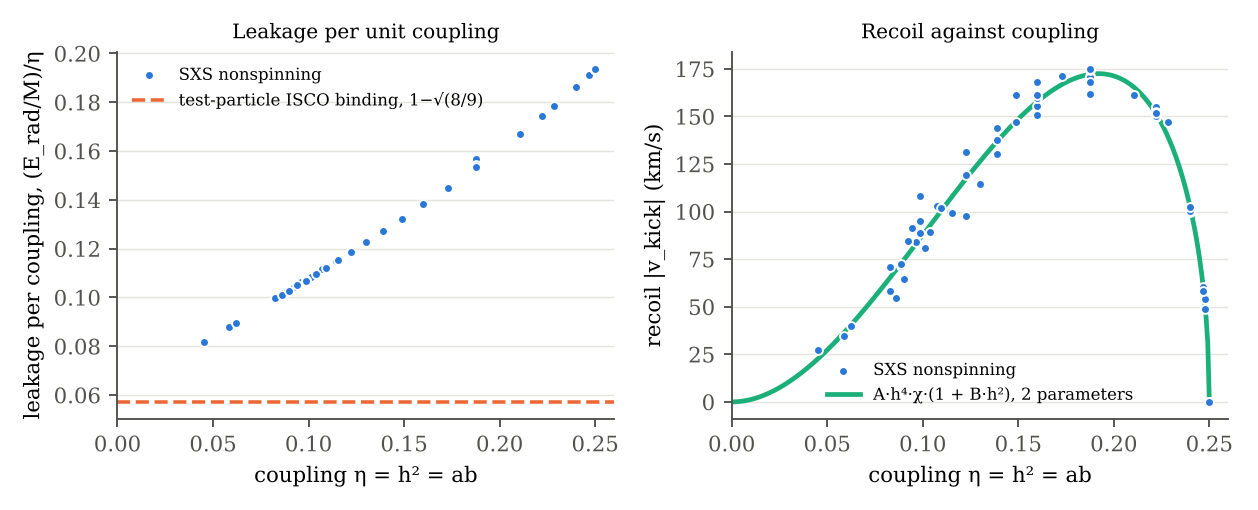
\includegraphics[width=\textwidth]{fig_sxs.png}
\caption{Non-spinning SXS runs. Left: leakage per unit coupling, $(\Erad/M)/\eta$, against
$\eta=h^2$, with the test-particle ISCO binding energy $1-\sqrt{8/9}$ (the $\eta\to0$ limit)
for comparison; the smallest $\eta$ in the sample is $0.045$. Right: recoil against $\eta$
with the two-parameter coupling-times-asymmetry form.}
\label{fig:sxs}
\end{figure}

\paragraph{What this shows.} Run as a procedure --- fix the instantiation from the
mechanism, then test --- the framework recovers known physics in partition language and
identifies which reading of the arc the domain uses. It does not supply new black-hole
physics, and nothing here claims it does.

% =====================================================================
\section{Withdrawn and corrected material}\label{sec:withdrawn}

\paragraph{The equipartition differential (withdrawn).} Revision 2 reported that the variance
explained by partition coordinates grows with distance from equipartition (SDSS density:
48-fold, Pearson $+0.86$; SXS: 13.7-fold, $+0.82$; SDSS gradient margin: $+0.87$). Two checks
show this should not be relied on.
\begin{enumerate}\sloppy
\item \emph{Null simulation.} With the SDSS bin edges of Revision 2 (0, 0.05, 0.10, 0.15,
0.20, 0.30, 0.50, 0.99), we simulated observables with no special role for asymmetry
(script \texttt{equipartition\_null\_test.py} in the reproducibility files). An observable that depends on $\chi$ with the same
strength everywhere gives an 88-fold increase in partial $R^2$ (Pearson $+0.94$); one
depending on $h$ gives 9.8-fold ($+0.84$); one depending on $\sin 2\chi$ gives 2.0-fold
($+0.27$). The main cause is the unequal bin widths: the last bin is about ten times wider
than the first, and within-bin predictor variance grows with the square of the width.
Basis-preference margins also grow with $\chi$ under these nulls (Pearson up to $+0.91$),
because all candidate bases agree to leading order near $\chi=0$. With only seven bins, a
Pearson coefficient has a 95\% interval of roughly $\pm0.7$. For the SXS bins of Revision 2 (0, 0.1, \dots, 0.65, 0.95), the width ratio is only 3, so bin width alone accounts for at most
part of the published SXS pattern; that claim fails on replication instead.
\item \emph{Replication.} On the current SXS catalog with the published bins, the ratio is
$1.8$ and the Pearson correlation $-0.17$; with equal-width bins, $1.6$ and $+0.11$.
\end{enumerate}
The SDSS results could not be re-tested here. In view of the null simulation, they are
withdrawn pending a re-analysis with equal-width bins and matched null controls. The
corresponding checklist item of Revision 2 is reversed (Section~\ref{sec:checklist}).

\paragraph{Removed heuristics.} The ``dimensional selection'' of Revision 2 (a one-parameter
family of metrics tuned so that one member reproduces an inverse-square law) fits a family to
a known target, which is the threshold-manufacturing pattern of~\cite{DeJesus2026CG}. The
``six Pythagorean powers'' classification had no testable content. The ``infinite half-step''
remark restated the boundary behaviour of Remark~\ref{rem:flat}. All three are removed. The
claimed pendulum and Kepler dynamics under a shared potential are also removed: dynamics are
supplied by the domain, not by the choice of kinetic metric~\cite{DeJesus2026EP}.

\paragraph{Corrected translation.} For the generating function, Revision 2 gave
$2\gd(\xi)\cosh\xi$ (rapidity) and $2\sqrt{2y}\arctan\sqrt{2y-1}$ (radial). These are the
forms of $\theta/h$, not of $G=\varphi/h=(\gd\xi+\tfrac\pi2)\cosh\xi$: they used the Fisher
angle $\theta$ where $2\varphi=\theta+\tfrac\pi2$ is required. They vanish at equipartition,
where $G=\pi/2$. The corrected forms are in Appendix~\ref{app:pairs}.

% =====================================================================
\section{Safeguards}\label{sec:safeguards}

\begin{enumerate}\sloppy
\item \textbf{The arc is automatic.} Every two-channel budget lies on it
(Proposition~\ref{prop:arc}); recurrence across domains is expected, not evidence.
\item \textbf{Chart contributions.} Divergences of $R$, $\xi$ or $y$ at $|\chi|\to1$ come
from the coordinates. In extracted potentials, the factor $(1-\chi^2)^{-1}$ is the chart and
the domain physics lives in the numerator~\cite{DeJesus2026EP}.
\item \textbf{Monotone equivalence.} All the coordinates are monotone functions of one
another, so rank-based statistics cannot tell them apart, and differences under polynomial
fits reflect curvature, not new information.
\item \textbf{Native composition.} A coordinate is native only if the domain's composition
law is additive in it, or its dynamics close in it.
\item \textbf{Orientation.} If the mechanism distinguishes the channels, use signed $\chi$
or $\xi$; $h$, $R$ and $y$ are blind to orientation.
\item \textbf{Closure.} Ask whether $a+b$ is conserved. If it is not, track the radius, and
remember that $R_{\rm act}$ grows with leakage alone.
\item \textbf{Declare the metric.} Any statement about distances or regions must say which
metric is meant (Remark~\ref{rem:flat}).
\item \textbf{Pre-commitment.} Fix the instantiation before comparing with data or targets.
\item \textbf{Normal forms are not tests.} Report an over-determination test before claiming
content.
\end{enumerate}

% =====================================================================
\section{Practical checklist}\label{sec:checklist}

\begin{enumerate}\sloppy
\item Identify the two channels and write the instantiation (Definition~\ref{def:inst})
before looking at data.
\item Check closure; if the budget leaks, measure $L$ independently.
\item Choose the native coordinate by composition or dynamics, not by appearance.
\item Translate with Table~\ref{tab:dictionary}; check that domains, bounds and
singularities correspond.
\item Classify: exact translation, partial correspondence, mixed object, or mismatch.
\item For empirical claims, use equal-width bins or binless methods, compare against a
shuffled or constant-effect null, and use held-out data.
\item Run at least one over-determination test and report it, including failures.
\end{enumerate}

% =====================================================================
\section{Epistemic tiers}\label{sec:tiers}
\begin{itemize}
\item \textbf{Tier 1}: Propositions~\ref{prop:arc}--\ref{prop:leak}; the metrics, the
inversion identity and the Gudermannian dictionary; the exponential-family duality; the
worked translations of Table~\ref{tab:pairs}; the e-fold form of the $\Lambda$CDM
partition. All are checked, symbolically or numerically, in \texttt{verify\_rev3.py}.
\item \textbf{Tier 2}: the SXS results of Section~\ref{sec:sxs}; the withdrawal analysis of
Section~\ref{sec:withdrawn}.
\item \textbf{Tier 3}: the constraint-type heuristic of Table~\ref{tab:constraints}; any
claim that two domains share physics because they share a reading of the arc.
\end{itemize}

% =====================================================================
\section{Conclusion}\label{sec:conclusion}

The binary partition gives every two-channel budget the same arc, and the dictionary of
Section~\ref{sec:dictionary} translates exactly between the coordinates people use on it.
That much was in Revision 2. What Revision 3 adds is a discipline for using it. The domain
instantiates the arc --- what the channels are, whether the budget is closed, whether the
coupling is realized, which coordinate composition makes additive, whether orientation
matters --- and it must do so before the comparison. Translations of known formulas are
normal forms. Claims need over-determination tests, and failed tests classify domains rather
than refuting the arc.

The SXS analysis shows what this looks like in practice: the coordinate predicted from the
physics gives the most compact description out of sample, the leakage law has an
independently known limit that the data are consistent with, and the recoil is compactly
written as coupling times asymmetry once the symmetry-required zeros are built in. The
empirical pattern that Revision 2 relied on is withdrawn, because a simple null reproduces
it. The guide is smaller as a result, and more useful.

\section*{Reproducibility}
\sloppy
\texttt{verify\_rev3.py} checks the Tier-1 identities symbolically or numerically.
\texttt{equipartition\_null\_test.py} reproduces the null simulation. \texttt{load.py},
\texttt{analyze.py} and \texttt{cv\_repeat.py}, with the plan in \texttt{sxs\_PREREGISTRATION.md},
reproduce Section~\ref{sec:sxs} from \texttt{simulations.json} of release v3.0.0 of the SXS
catalog data (\texttt{sxs-collaboration/sxscatalogdata}), which \texttt{fetch\_data.py}
downloads and checks against a fixed checksum. All files are in the folder
\texttt{two-face-problem-rev3/} of the repository
\url{https://github.com/innerlightr-wq/constraint-geometry-domain-physics}.

\section*{Acknowledgments}
Claude (Anthropic) assisted with verification, data analysis and manuscript preparation for
this revision. All conceptual development, research direction, interpretation and final
responsibility rest with the author.

\appendix
% =====================================================================
\section{Worked translations in full}\label{app:pairs}

\paragraph{Fermi--Dirac and logistic.} Take $a$ to be the vacant fraction and $b=f$ the
occupied one. Then $f(x)=1/(e^x+1)=(1-\tanh\xi)/2$ with $\xi=x/2$, $a=(1+\tanh\xi)/2$, and
$\log\frac{a}{b}=2\xi=x$; with the opposite assignment, $\xi\to-\xi$. In the Fisher angle,
$f=(1-\sin\theta)/2$ with $\theta=\gd(x/2)$; in the radial coordinate,
$f=(1-\sqrt{1-1/(2y)})/2$ with $y=\tfrac12\cosh^2(x/2)$.

\paragraph{Mercator.} Latitude $\phi_{\rm lat}$ maps to the Mercator ordinate
$\psi=\ln(\sec\phi_{\rm lat}+\tan\phi_{\rm lat})=\gd^{-1}(\phi_{\rm lat})$, and
$\psi=\mathrm{arccosh}(\sec\phi_{\rm lat})$ for $\phi_{\rm lat}\ge0$.

\paragraph{Bernoulli Fisher information.} $I_F(p)=1/(p(1-p))=1/h^2=4R=8y
=4\sec^2\theta=4\cosh^2\xi$.

\paragraph{Aberration.} With $\beta=\tanh\xi$ and the convention
$\cos\theta'=(\cos\theta+\beta)/(1+\beta\cos\theta)$,
$\tan(\theta'/2)=\sqrt{(1-\beta)/(1+\beta)}\,\tan(\theta/2)=e^{-\xi}\tan(\theta/2)$, and
$e^{-\xi}=\sqrt{2y}-\sqrt{2y-1}$.

\paragraph{VSWR.} $\mathrm{VSWR}=(1+|\Gamma|)/(1-|\Gamma|)=e^{2|\xi|}
=(\sqrt{2y}+\sqrt{2y-1})^2$. For a resistive load,
$\Gamma=(Z-Z_0)/(Z+Z_0)=\tanh(\tfrac12\ln(Z/Z_0))$, so $\xi=\tfrac12\ln(Z/Z_0)$ and
$\mathrm{VSWR}=\max(Z/Z_0,Z_0/Z)$.

\paragraph{Altitude integrals.} $I(\alpha)=\int_0^1[x(1-x)]^{\alpha/2}dx
=B(\tfrac\alpha2+1,\tfrac\alpha2+1)$; $I(1)=\pi/8$, $I(-1)=\pi$. In rapidity,
$I(\alpha)=2^{-(\alpha+1)}\int_{-\infty}^\infty\sech^{\alpha+2}\xi\,d\xi$.

\paragraph{Generating function (corrected).} Since $\int_0^1 h^{2m}dx=B(m+1,m+1)$,
\[
G(t)=\sum_{m\ge0}t^m\!\int_0^1 h(x)^{2m}dx=\int_0^1\frac{dx}{1-t\,x(1-x)}
=\frac{4\arcsin(\sqrt t/2)}{\sqrt{t(4-t)}} .
\]
Setting $a=t/4$, $\varphi=\arcsin\sqrt a$ and $h_a=\sqrt{a(1-a)}$ gives $G=\varphi/h_a$. Since
$\varphi=\tfrac12(\theta+\tfrac\pi2)$ and $h=\tfrac12\sech\xi$,
\[
G=\big(\gd\xi+\tfrac\pi2\big)\cosh\xi=\sqrt{2y}\,\big(\pm\arctan\sqrt{2y-1}+\tfrac\pi2\big),
\]
with the sign of $\chi=2a-1$. At equipartition $G=\pi/2$. Revision 2 gave $2\gd(\xi)\cosh\xi$
and $2\sqrt{2y}\arctan\sqrt{2y-1}$, which are the forms of $\theta/h$, not of $G$.

\paragraph{Langevin and Bose--Einstein.} $\coth x-1/x$ combines a hyperbolic term and a
reciprocal term, and no single coordinate makes it simple. $1/(e^x-1)$ is unbounded and is
not a share of a two-channel budget.

\bibliographystyle{unsrtnat}
\bibliography{references}

\end{document}
